\newpage
\thispagestyle{empty}

\newpar
Ted Sundstrom \\
Department of Mathematics \\
Grand Valley State University \\
Allendale, MI  49401 \\
mathreasoning@gmail.com


\quarter
\newpar
\emph{Mathematical Reasoning: Writing and Proof}

\noindent
\copyright \the\year by Ted Sundstrom

\newpar
Previous versions of this book were published by Pearson Education, Inc.

\half
\newpar
\textbf{\huge{License}}

\newpar
%This work is licensed under the Creative Commons Attribution-NonCommercial-No Derivative Works
%3.0 Unported License. The graphic
%\begin{center}
%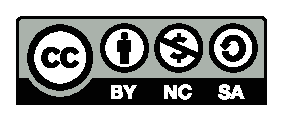
\includegraphics{CClicense.eps}
%%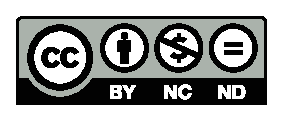
\includegraphics{CC-by-nc-nd.eps}
%\end{center}
%that appears throughout the text shows that the work is licensed with the Creative Commons, that
%the work may be used for free by any party so long as attribution is given to the author.  In addition, this work may not be altered or transformed and no party may
%sell this work for profit. Full details may be found by visiting
%\begin{center}
%http://creativecommons.org/licenses/by-nc-nd/3.0/
%\end{center}
%or sending a letter to Creative Commons, 444 Castro Street, Suite 900, Mountain View, California,
%94041, USA.


This work is licensed under the Creative Commons Attribution-NonCommercial-ShareAlike
3.0 Unported License. The graphic
\begin{center}
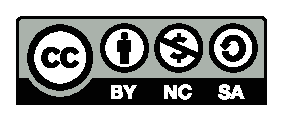
\includegraphics{CClicense.eps}
\end{center}
that appears throughout the text shows that the work is licensed with the Creative Commons, that
the work may be used for free by any party so long as attribution is given to the author(s), that the
work and its derivatives are used in the spirit of ``share and share alike,'' and that no party other than the author(s) may
sell this work or any of its derivatives for profit. Full details may be found by visiting
\begin{center}
\href{http://creativecommons.org/licenses/by-nc-sa/3.0/}%
{http://creativecommons.org/licenses/by-nc-sa/3.0/}
\end{center}
or sending a letter to Creative Commons, 444 Castro Street, Suite 900, Mountain View, California,
94041, USA.

\newpage
\thispagestyle{empty}
$ $
\endinput

\endinput
